% Copyright 2004 by Till Tantau <tantau@users.sourceforge.net>.
%
% In principle, this file can be redistributed and/or modified under
% the terms of the GNU Public License, version 2.
%
% However, this file is supposed to be a template to be modified
% for your own needs. For this reason, if you use this file as a
% template and not specifically distribute it as part of a another
% package/program, I grant the extra permission to freely copy and
% modify this file as you see fit and even to delete this copyright
% notice. 

\documentclass{beamer}

\usepackage{tikz}
\usetikzlibrary{positioning}
\usetikzlibrary{matrix,decorations.pathreplacing,calc}
\usepackage{pgfplots}
\pgfplotsset{compat=1.10}
\usepackage{amsthm,amsmath,amssymb,amsfonts}
\usepackage{graphicx}

\usepackage[spanish]{babel}
\usepackage[utf8]{inputenc}
\usepackage[T1]{fontenc}

\usepackage{neuralnetwork}
\usepackage{xcolor}

\usepackage{caption}
\usepackage{subcaption}
%\usepackage[demo]{graphicx}

\usepackage{wrapfig}



\tikzset{basic/.style={draw,fill=blue!20,text width=1em,text badly centered}}
\tikzset{input/.style={basic,circle}}
\tikzset{weights/.style={basic,rectangle}}
\tikzset{functions/.style={basic,circle,fill=blue!10}}
\tikzstyle{arrow}=[draw, -latex]

\makeatletter
\newsavebox{\measure@tikzpicture}
\NewEnviron{scaletikzpicturetowidth}[1]{%
  \def\tikz@width{#1}%
  \def\tikzscale{1}\begin{lrbox}{\measure@tikzpicture}%
  \BODY
  \end{lrbox}%
  \pgfmathparse{#1/\wd\measure@tikzpicture}%
  \edef\tikzscale{\pgfmathresult}%
  \BODY
}
\makeatother



\pgfkeys{tikz/mymatrixenv/.style={decoration=brace,every left delimiter/.style=    {xshift=3pt},every right delimiter/.style={xshift=-3pt}}}
\pgfkeys{tikz/mymatrix/.style={matrix of math nodes,left delimiter=[,right delimiter=    {]},inner sep=2pt,column sep=1em,row sep=0.5em,nodes={inner sep=0pt}}}
\pgfkeys{tikz/mymatrixbrace/.style={decorate,thick}}

\newcommand\mymatrixbraceoffseth{0.5em}
 \newcommand\mymatrixbraceoffsetv{0.2em}
 
\newcommand*\mymatrixbracetop[4][mtr]{
\draw[mymatrixbrace] ($(#1.north west)!(#1-1-#2.north west)!(#1.north east)+(0,\mymatrixbraceoffsetv)$)
    -- node[above=2pt] {#4} 
    ($(#1.north west)!(#1-1-#3.north east)!(#1.north east)+(0,\mymatrixbraceoffsetv)$);
}

\newcommand*\mymatrixbraceleft[4][mtr]{
 \draw[mymatrixbrace] ($(#1.north east)!(#1-#2-1.north east)!(#1.south east)+    (\mymatrixbraceoffseth,0)$)
    -- node[right=2pt] {#4} 
     ($(#1.north east)!(#1-#3-1.south east)!(#1.south east)+    (\mymatrixbraceoffseth,0)$);
}



\usepackage{pdfpages}

% There are many different themes available for Beamer. A comprehensive
% list with examples is given here:
% http://deic.uab.es/~iblanes/beamer_gallery/index_by_theme.html
% You can uncomment the themes below if you would like to use a different
% one:
%\usetheme{AnnArbor}
%\usetheme{Antibes}
%\usetheme{Bergen}
%\usetheme{Berkeley}
%\usetheme{Berlin}
%\usetheme{Boadilla}
%\usetheme{boxes}
%\usetheme{CambridgeUS}
%\usetheme{Copenhagen}
%\usetheme{Darmstadt}
%\usetheme{default}
%\usetheme{Frankfurt}
%\usetheme{Goettingen}
%\usetheme{Hannover}
%\usetheme{Ilmenau}
%\usetheme{JuanLesPins}
%\usetheme{Luebeck}
\usetheme{Madrid}
%\usetheme{Malmoe}
%\usetheme{Marburg}
%\usetheme{Montpellier}
%\usetheme{PaloAlto}
%\usetheme{Pittsburgh}
%\usetheme{Rochester}
%\usetheme{Singapore}
%\usetheme{Szeged}
%\usetheme{Warsaw}

\title{Wordnet y Deep Learning: Una posible
unión}

% A subtitle is optional and this may be deleted
\subtitle{ 
Trabajo de fin de grado}

\author{Raquel Leandra Pérez Arnal}
% - Give the names in the same order as the appear in the paper.
% - Use the \inst{?} command only if the authors have different
%   affiliation.

 % Your name

\author[Raquel Leandra Pérez Arnal]{\textbf {Autor: Raquel Leandra Pérez Arnal\\ \footnotesize Directores: Dario Garcia Gasulla y Claudio Ulises Cortés
García}}
\institute[FME] % Your institution as it will appear on the bottom of every slide, may be shorthand to save space
{
Universidad Politécnica de Cataluña \\ % Your institution for the title page
Facultad de Matemáticas y Estadística \\
\medskip
\textit{raquelpa93@gmail.com} % Your email address
}

% - Use the \inst command only if there are several affiliations.
% - Keep it simple, no one is interested in your street o.

\date{22/01/18}
% - Either use conference name or its abbreviation.
% - Not really informative to the audience, more for people (including
%   yourself) who are reading the slides online

\subject{Theoretical Computer Science}
% This is only inserted into the PDF information catalog. Can be left
% out. 

% If you have a file called "university-logo-filename.xxx", where xxx
% is a graphic format that can be processed by latex or pdflatex,
% resp., then you can add a logo as follows:

% \pgfdeclareimage[height=0.5cm]{university-logo}{university-logo-filename}
% \logo{\pgfuseimage{university-logo}}

% Delete this, if you do not want the table of contents to pop up at
% the beginning of each subsection:
\setbeamertemplate{caption}[numbered]
%\AtBeginSubsection[]
%{
%  \begin{frame}<beamer>{}
%    \tableofcontents[currentsection,currentsubsection]
%  \end{frame}
%}
\AtBeginSection[]{%
  \begin{frame}<beamer>
    \frametitle{}
    %\tableofcontents[sectionstyle=show/hide,subsectionstyle=hide/show/hide]
    \tableofcontents[currentsection,currentsubsection]
  \end{frame}
  \addtocounter{framenumber}{-1}% If you don't want them to affect the slide number
}

% Let's get started
\begin{document}

\begin{frame}
  \titlepage
\end{frame}
\setcounter{tocdepth}{1}
\begin{frame}{Tabla de contenidos}
  \tableofcontents
  % You might wish to add the option [pausesections]
\end{frame}

% Section and subsections will appear in the presentation overview
% and table of contents.
\section{Conocimientos Previos}

\subsection{Redes Neuronales}
\begin{frame}{Una Neurona}
\begin{figure}
\centering
 \begin{tikzpicture}
        \node[functions] (center) {$f$};
        \node[below of=center,font=\scriptsize,text width=4em] {Función de activación};

        \node[right of=center] (right) {};
            \path[draw,arrow] (center) -- (right);
        \node[functions,left=3em of center,text width=3em ] (left) {$\sum w_i x_i$};
            \path[draw,arrow] (left) -- (center);
        \node[weights,left=3em of left] (2) {$w_2$} -- (2) node[input,left of=2] (l2) {$x_2$};
            \path[draw,arrow] (l2) -- (2);
            \path[draw,arrow] (2) -- (left);
        \node[below of=2] (dots) {$\vdots$} -- (dots) node[left of=dots] (ldots) {$\vdots$};
        \node[weights,below of=dots] (n) {$w_n$} -- (n) node[input,left of=n] (ln) {$x_n$};
            \path[draw,arrow] (ln) -- (n);
            \path[draw,arrow] (n) -- (left);
        \node[weights,above of=2] (1) {$w_1$} -- (1) node[input,left of=1] (l1) {$x_1$};
            \path[draw,arrow] (l1) -- (1);
            \path[draw,arrow] (1) -- (left);
        \node[weights,above of=1] (0) {$w_0$} -- (0) node[input,left of=0] (l0) {$1$};
            \path[draw,arrow] (l0) -- (0);
            \path[draw,arrow] (0) -- (left);
        \node[below of=ln,font=\scriptsize] {Pesos};
        \node[below of=n,font=\scriptsize] { Entrada};
    \end{tikzpicture}
    \caption{Ejemplo de una neurona}
\end{figure}
\end{frame}

\begin{frame}[fragile]{Red Neuronal}
\begin{figure}[H]
\begin{center}
\begin{neuralnetwork}[height=5]
		\newcommand{\nodetextclear}[2]{}
		\newcommand{\nodetextx}[2]{$x_#2$}
		\newcommand{\nodetexty}[2]{$y_#2$}
		\newcommand{\nodetextw}[2]{$a_#2^#1$}
		\inputlayer[count=3, bias=true, title=Capa \\de entrada, text=\nodetextx]
		\hiddenlayer[count=4, bias=true, title=Capa \\ oculta 1, text=\nodetextw] \linklayers
		\hiddenlayer[count=4, bias=true, title=Capa \\ oculta 2, text=\nodetextw] \linklayers
		\outputlayer[count=3, title=Capa\\ de salida, text=\nodetexty] \linklayers
	
		\end{neuralnetwork}	
\end{center}
\caption{Ejemplo de red neuronal compuesta por capas completas}
\end{figure}
\end{frame}



\subsection{Redes Convolucionales}

%\begin{frame}{Redes Convolucionales}
%\begin{block}
%Una convol
%\end{block}
%\end{frame}

\begin{frame}[fragile]{Redes Convolucionales}

\begin{figure}[H]

\begin{center}
%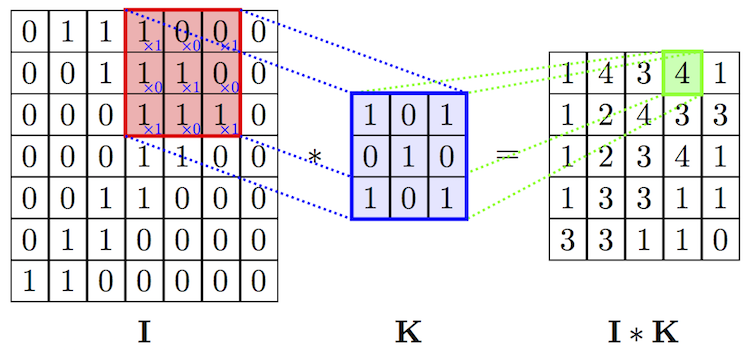
\includegraphics[width = 0.5\textwidth]{Images/convolve.png} 
\begin{tikzpicture}

	\matrix (mtr) [matrix of nodes,row sep=-\pgflinewidth, nodes={draw}]
	{
		0 & 1 & 1 & |[fill=red!30]| 1 & |[fill=red!30]| 0 & |[fill=red!30]| 0 & 0\\
		0 & 0 & 1 & |[fill=red!30]| 1 & |[fill=red!30]| 1 & |[fill=red!30]| 0 & 0\\
		0 & 0 & 0 & |[fill=red!30]| 1 & |[fill=red!30]| 1 & |[fill=red!30]| 1 & 0\\
		0 & 0 & 0 & 1 & 1 & 0 & 0\\
		0 & 0 & 1 & 1 & 0 & 0 & 0\\
		0 & 1 & 1 & 0 & 0 & 0 & 0\\
		1 & 1 & 0 & 0 & 0 & 0 & 0\\
	};

	\draw[very thick, red] (mtr-1-4.north west) rectangle (mtr-3-6.south east);

	\node [below= of mtr-5-4.south] (lm) {$\bf I$};

	\node[right = 0.2em of mtr] (str) {$*$};

	\matrix (K) [right=0.2em of str,matrix of nodes,row sep=-\pgflinewidth, nodes={draw, fill=blue!30}]
	{
		1 & 0 & 1 \\
		0 & 1 & 0 \\
		1 & 0 & 1 \\
	};
	\node [below = of K-3-2.south] (lk) {$\bf K$};

	\node [right = 0.2em of K] (eq) {$=$};

	\matrix (ret) [right=0.2em of eq,matrix of nodes,row sep=-\pgflinewidth, nodes={draw}]
	{
		1 & 4 & 3 & |[fill=green!30]| 4 & 1\\
		1 & 2 & 4 & 3 & 3\\
		1 & 2 & 3 & 4 & 1\\
		1 & 3 & 3 & 1 & 1\\
		3 & 3 & 1 & 1 & 0\\
	};
	\node [below = of ret-4-3.south] (lim) {${\bf I} * {\bf K}$};

	\draw[very thick, green] (ret-1-4.north west) rectangle (ret-1-4.south east);

	\draw[densely dotted, blue, thick] (mtr-1-4.north west) -- (K-1-1.north west);
	\draw[densely dotted, blue, thick] (mtr-3-4.south west) -- (K-3-1.south west);
	\draw[densely dotted, blue, thick] (mtr-1-6.north east) -- (K-1-3.north east);
	\draw[densely dotted, blue, thick] (mtr-3-6.south east) -- (K-3-3.south east);

	\draw[densely dotted, green, thick] (ret-1-4.north west) -- (K-1-1.north west);
	\draw[densely dotted, green, thick] (ret-1-4.south west) -- (K-3-1.south west);
	\draw[densely dotted, green, thick] (ret-1-4.north east) -- (K-1-3.north east);
	\draw[densely dotted, green, thick] (ret-1-4.south east) -- (K-3-3.south east);

	\matrix (K) [right=0.2em of str,matrix of nodes,row sep=-\pgflinewidth, nodes={draw, fill=blue!10}]
	{
		1 & 0 & 1 \\
		0 & 1 & 0 \\
		1 & 0 & 1 \\
	};

	\draw[very thick, blue] (K-1-1.north west) rectangle (K-3-3.south east);

	\node[anchor=south east, inner sep=0.01em, blue] at (mtr-1-4.south east) (xx) {\scalebox{.5}{$\times 1$}};
	\node[anchor=south east, inner sep=0.01em, blue] at (mtr-1-5.south east) (xx) {\scalebox{.5}{$\times 0$}};
	\node[anchor=south east, inner sep=0.01em, blue] at (mtr-1-6.south east) (xx) {\scalebox{.5}{$\times 1$}};
	\node[anchor=south east, inner sep=0.01em, blue] at (mtr-2-4.south east) (xx) {\scalebox{.5}{$\times 0$}};
	\node[anchor=south east, inner sep=0.01em, blue] at (mtr-2-5.south east) (xx) {\scalebox{.5}{$\times 1$}};
	\node[anchor=south east, inner sep=0.01em, blue] at (mtr-2-6.south east) (xx) {\scalebox{.5}{$\times 0$}};
	\node[anchor=south east, inner sep=0.01em, blue] at (mtr-3-4.south east) (xx) {\scalebox{.5}{$\times 1$}};
	\node[anchor=south east, inner sep=0.01em, blue] at (mtr-3-5.south east) (xx) {\scalebox{.5}{$\times 0$}};
	\node[anchor=south east, inner sep=0.01em, blue] at (mtr-3-6.south east) (xx) {\scalebox{.5}{$\times 1$}};

\end{tikzpicture}
\end{center}
\centering
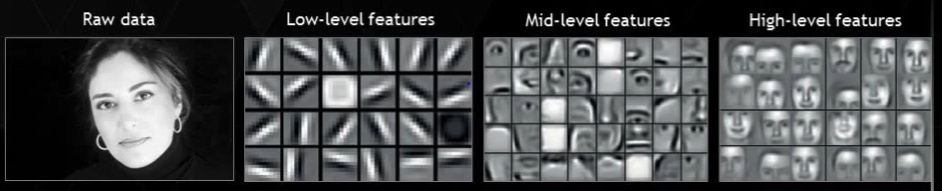
\includegraphics[width = 0.8\textwidth]{Images/deepConcept.png} 
\caption{Ejemplo de convolución y de feature}
\end{figure}

\end{frame}

\subsection{Transfer Learning}
\begin{frame}{Transfer Learning}

\begin{block}{Definición}
\textbf{Transfer learning} es el campo de estudio que reutiliza el lenguaje de representación de un problema (que llamaremos problema origen o \textit{Source}) para resolver otro (que llamaremos objetivo o \textit{Target}). 

\begin{itemize}
\item \textbf{Fine Tuning}
\item \textbf{Feature Extraction}
\end{itemize}
\end{block}

\begin{figure}[H]
\centering
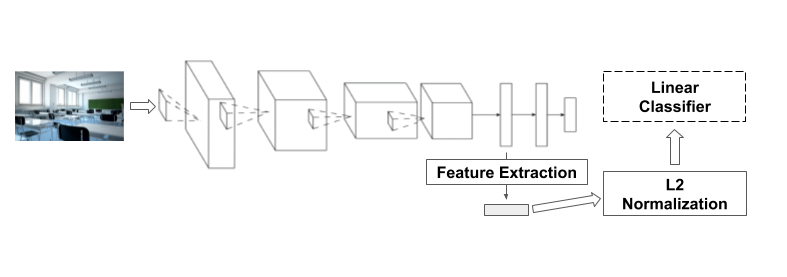
\includegraphics[width = 0.8\textwidth]{Images/basecrop.png} 
\caption{Estructura básica que se suele utilizar en \textit{feature extraction}
\label{fig:base}}
\end{figure}
\end{frame}

\begin{frame}{Importancia del \textit{Transfer Learning}}
\begin{itemize}
\item Permite aplicar métodos de \textit{Deep Learning} a conjuntos de datos de cualquier tamaño.
\item No requiere tiempo y poder computacional.
\item No requiere ajustar los hiper-parámetros. 
\end{itemize}
\end{frame}

\section{Trabajo Relacionado}

\subsection{Full-Network Embedding}

\begin{frame}{Full-Network Embedding}
Partes del algoritmo: 
\begin{itemize}
\item Fordward Pass
\item Spatial Pooling
\item Feature Standarization
\item Feature Discretization
\end{itemize}
\begin{figure}[h]
\label{fig:fne}
\centering
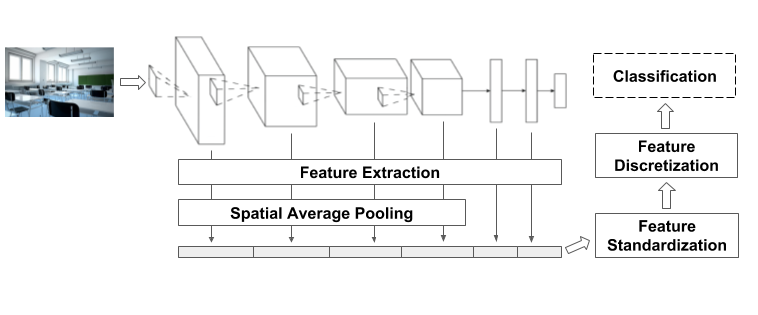
\includegraphics[width = 0.8\textwidth]{Images/cropfne.png} 
\caption{Estructura del \textit{full-network embedding}\label{fig:fnediagram}}
\end{figure}

\end{frame}
\subsection{Wordnet}

\begin{frame}{Wordnet}
\begin{figure}[ht] 
	\centering
	\begin{subfigure}[b]{0.3\textwidth}
	\begin{tikzpicture}[
    grow=right,
    level 1/.style={sibling distance=3cm,level distance=2cm},
    edge from parent/.style={<->, draw, >=latex},
    edge from parent path={(\tikzparentnode.east) -- (\tikzchildnode.west)},
    punkt/.style={rectangle, rounded corners, shade, top color=blue!20, bottom color=blue!20, draw=blue!40!black!60, very
    thick }
    ]

\node[punkt] {Pelo}
    %Lower part lv1
    %Upper part, lv1
    child {
        node[punkt] {Cabello}
    };
\end{tikzpicture}
		\caption{Ejemplo de Sinónimos \label{fig:sinonimos}}
	\end{subfigure}
	\begin{subfigure}[b]{0.3\textwidth}
		\begin{tikzpicture}[sibling distance=5em,
  every node/.style = {shape=rectangle, rounded corners,
    draw, align=center,
    top color=blue!20, bottom color=blue!20},
    edge from parent/.style={draw,-latex}
    ]
  \node {Ser Vivo}
  	child{ node {Mamífero}
    	child{ node {Perro}}
    	child{node {Gato}}
    };
\end{tikzpicture}
		\caption{Ejemplo de Hipónimos \label{fig:hiponimos}}
	\end{subfigure}
	\begin{subfigure}[b]{0.3\textwidth}
		\begin{tikzpicture}[sibling distance=5em,
  every node/.style = {shape=rectangle, rounded corners,
    draw, align=center,
    top color=blue!20, bottom color=blue!20},
    edge from parent/.style={<-, draw,>=latex}
    ]
  \node {Perro}
    	child{node {Dálmata}}
    	child{node {Cachorro}
    	};
\end{tikzpicture}
		\caption{Ejemplo de Hiperónimos \label{fig:hiperonimos}}
	\end{subfigure}    
	\caption{Ejemplo de las relaciones sintácticas de Wordnet}   
\end{figure}
\end{frame}

\subsection{Imagenet}

\begin{frame}{Imagenet}
\begin{figure}[h]
\label{fig:fne}
\centering
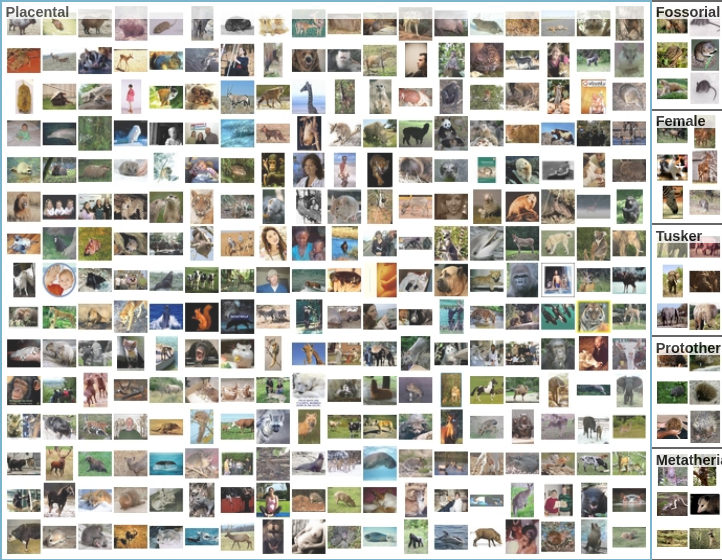
\includegraphics[width = 0.55\textwidth]{Images/imagenet/mammal.png} 
\end{figure}

En nuestro caso hemos utilizado el subconjunto del reto de \textit{Imagenet}2012: 

\begin{center}
\begin{tabular}{l|l|l|}
              & Cantidad & Clases \\ \hline
 Entrenamiento & 1.2 M    & 1000   \\ \hline
 Validación    & 50,000   & 1000   \\ \hline
\end{tabular}

\end{center}



\end{frame}
\section{Enfoque}

\begin{frame}[fragile]{Datos iniciales}


\begin{figure}[H]
\label{}
\centering
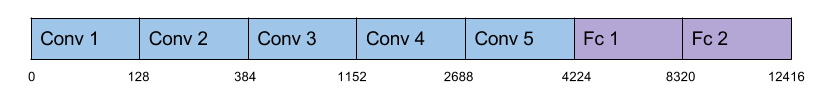
\includegraphics[width = \textwidth]{Images/croplayer.png} 
%\caption{La disposición de las características por capas \label{fig:featuresperlayer}}

\begin{center}
\begin{tikzpicture}[mymatrixenv]

	\matrix (mtr) [matrix of nodes,column sep=-\pgflinewidth, row sep=-\pgflinewidth,  nodes={draw,
      minimum height=0.5cm,
      anchor=center,
      text width=0.5cm,
      align=center,
      inner sep=0pt
    }]
	{
		|[fill=blue!30]| 1 & |[fill=blue!30]| 1 & |[fill=blue!30]| -1 & |[fill=blue!30]| 1 & |[fill=blue!30]| 0 & |[fill=blue!30]| 0 & |[fill=blue!30]| -1\\
		0 & 0 & -1 & -1 & -1 & 0 & 0\\
		0 & 0 & 0 & 1 & -1 & -1 & 0\\
		|[fill=green!30]| 1 & |[fill=green!30]| 1 & |[fill=green!30]| -1 & |[fill=green!30]| 1 & |[fill=green!30]| -1 & |[fill=green!30]| 0 & |[fill=green!30]| 0\\
		0 & 0 & -1 & 1 & 0 & 0 & 0\\
		0 & -1 & 1 & 0 & 0 & 0 & 1\\
		|[fill=blue!30]| 1 & |[fill=blue!30]| 1 & |[fill=blue!30]| -1 & |[fill=blue!30]| -1 & |[fill=blue!30]| -1 & |[fill=blue!30]| 0 & |[fill=blue!30]| 0\\
		-1 & -1 & 0 & 0 & 0 & 0 & 0\\
	};

	\draw[very thick, blue] (mtr-1-1.north west) rectangle (mtr-1-7.south east);
	\draw[very thick, green] (mtr-4-1.north west) rectangle (mtr-4-7.south east);
	\draw[very thick, blue] (mtr-7-1.north west) rectangle (mtr-7-7.south east);
    \node[left=12pt of mtr-1-1] (left-1) {ser vivo};
    \node[left=12pt of mtr-7-1] (left-3) {ser vivo};
    \node[left=12pt of mtr-4-1] (left-2) {mamífero};
    
    \mymatrixbracetop{1}{7}{\textit{features}}
 \mymatrixbraceleft{1}{8}{muestras}


\end{tikzpicture}
\end{center}
\caption{Muestra de una sección del embedding (de tamaño total  50,000 x 12,416). 
\label{fig:muestrasynsets}
}
\end{figure}

\end{frame}

\subsection{Objetivos}

\begin{frame}[fragile]{Objetivos}

\begin{itemize}
\item Analizar el \textit{embedding} dado y el comportamiento de las \textit{features} en las distintas capas.
\item Analizar si hay alguna relación entre el \textit{embedding} y los \textit{synsets} seleccionados.
\end{itemize}


\begin{figure}[H]
\centering
\begin{subfigure}{.5\textwidth}
  \centering
  %\includegraphics[width=.4\linewidth]{image1}
\begin{tikzpicture}[sibling distance=6em,level distance=3em,
  every node/.style = {shape=rectangle, rounded corners,
    draw, align=center,
    top color=cyan!20, bottom color=cyan!20},
    edge from parent/.style={draw,-latex}
    ]
  \node {Ser Vivo}
  	child{ node {Mamífero}
    	child{ node {Perro}
			child{node {Perro de caza}    	
    		}
    	}
    };
\end{tikzpicture}
  %\caption{Seres vivos}
  %\label{fig:sub1}
\end{subfigure}%
\begin{subfigure}{.5\textwidth}
  \centering
  \begin{tikzpicture}[sibling distance=5em,level distance=3em,
  every node/.style = {shape=rectangle, rounded corners,
    draw, align=center,
    top color=red!20, bottom color=red!20},
    edge from parent/.style={draw,-latex}
    ]
  \node {Artefacto}
  	child{ node {Instrumento}
    	child{ node {Transporte}
			child{node {Vehículo}    	
    		}
    	}
    };
\end{tikzpicture}
 % \caption{Objetos}
 % \label{fig:sub2}
\end{subfigure}
\caption{Conjuntos de synsets que estudiaremos \label{fig:synsets}}
\end{figure}


\end{frame}

\subsection{Estadísticas e Hipótesis iniciales}

\begin{frame}{Estadísticas del embedding}

\begin{figure}[h] 
	\centering
	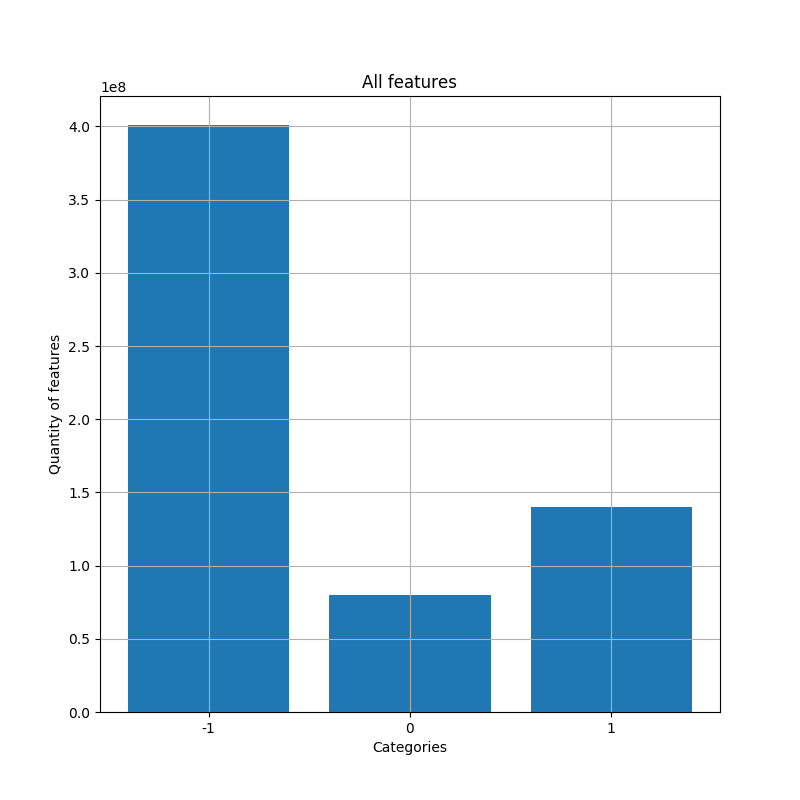
\includegraphics[width=0.6\textwidth] {Images/plots/25/quantity_of_features_bar.png}
	\caption{ Cantidad de \textit{features} de cada categoría
	\label{fig:totalfeatures}}
\end{figure}
\end{frame}

\begin{frame}{Estadísticas del embedding}

\begin{figure}[ht] 
	\centering
	\begin{subfigure}[b]{0.32\textwidth}
		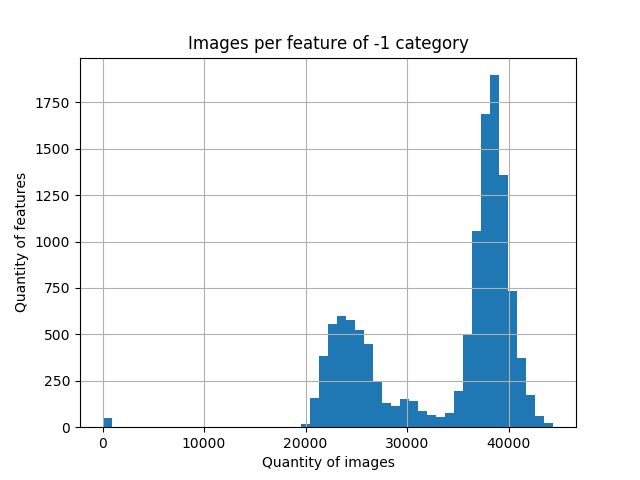
\includegraphics[width=\textwidth] {Images/plots/25/Images_per_feature_of_-1_category.png}
		\caption{Categoría -1}
	\end{subfigure}
	\begin{subfigure}[b]{0.32\textwidth}
		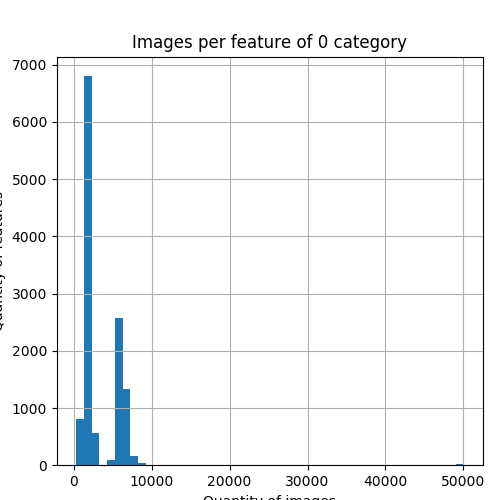
\includegraphics[width=\textwidth]  {Images/plots/25/Images_per_feature_of_0_category.png}
		\caption{Categoría 0}
	\end{subfigure}
	\begin{subfigure}[b]{0.32\textwidth}
		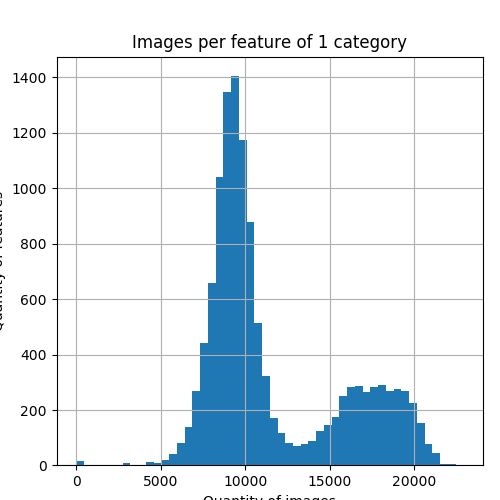
\includegraphics[width=\textwidth]  {Images/plots/25/Images_per_feature_of_1_category.png}
		\caption{Categoría 1}
	\end{subfigure}       
	\caption{Distribución del número de \textit{features} con los distintos valores categóricos, para las 50,000 imágenes  \label{fig:imagesperfeature}}
\end{figure}
\end{frame}

\begin{frame}{Distribución de los synsets en el embeding}


\begin{figure}[H] 
	\centering
	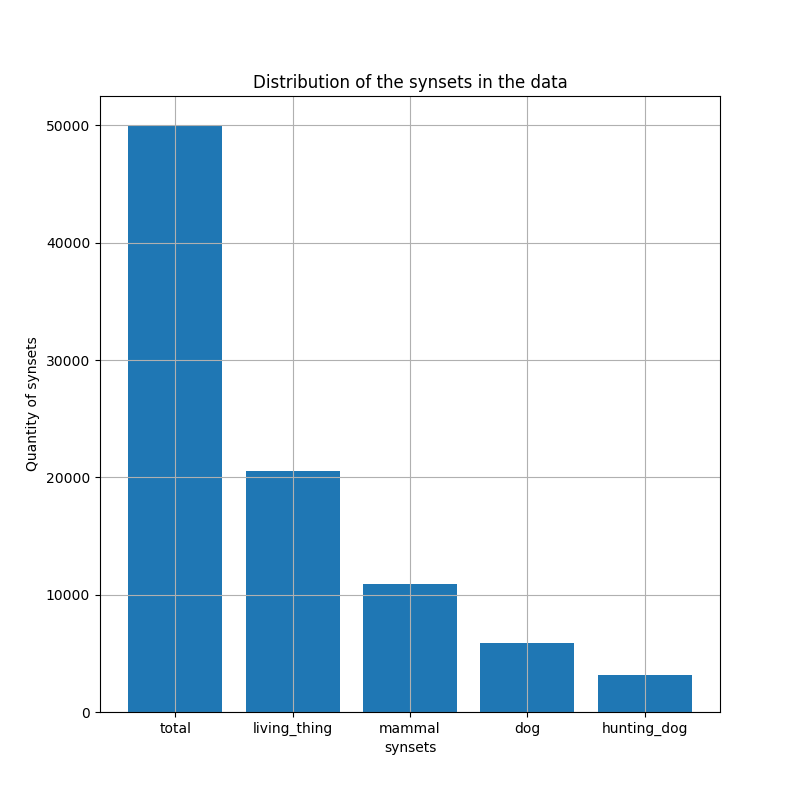
\includegraphics[width=0.8\textwidth] {Images/plots/25/distribution_of_synsets_bar.png}
		\caption{ Cantidad de imágenes de cada \textit{synset} respecto al embedding total
	\label{fig:totalsynsets}}
\end{figure}
\end{frame}

\begin{frame}{Hipótesis}
\begin{enumerate}
\item \label{h1} Las características se distribuyen de diferente manera en las capas convolucionales y los completos. 
\item \label{h3} La cantidad de \textit{features} representativas aumenta con la profundidad.
\item \label{h2} Cuanto más concreto es un \textit{synset}, más \textit{features} representativas.
\item \label{h4} Se puede ver una relación entre los embeddings de synsets hipónimos. 
\end{enumerate}

\end{frame}

\section{Análisis}

\subsection{De Wordnet a Full-Network Embedding}

\begin{frame}{Distribución por tipo de capa}

\begin{figure}[ht] 
	\centering
	\begin{subfigure}[b]{0.32\textwidth}
		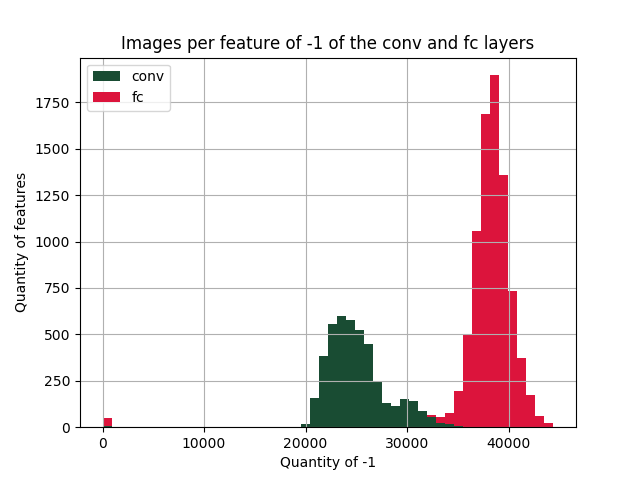
\includegraphics[width=\textwidth] {Images/plots/25/Images_per_feature_of_-1_category_all_layers.png}
		\caption{Categoría -1}
	\end{subfigure}
	\begin{subfigure}[b]{0.32\textwidth}
		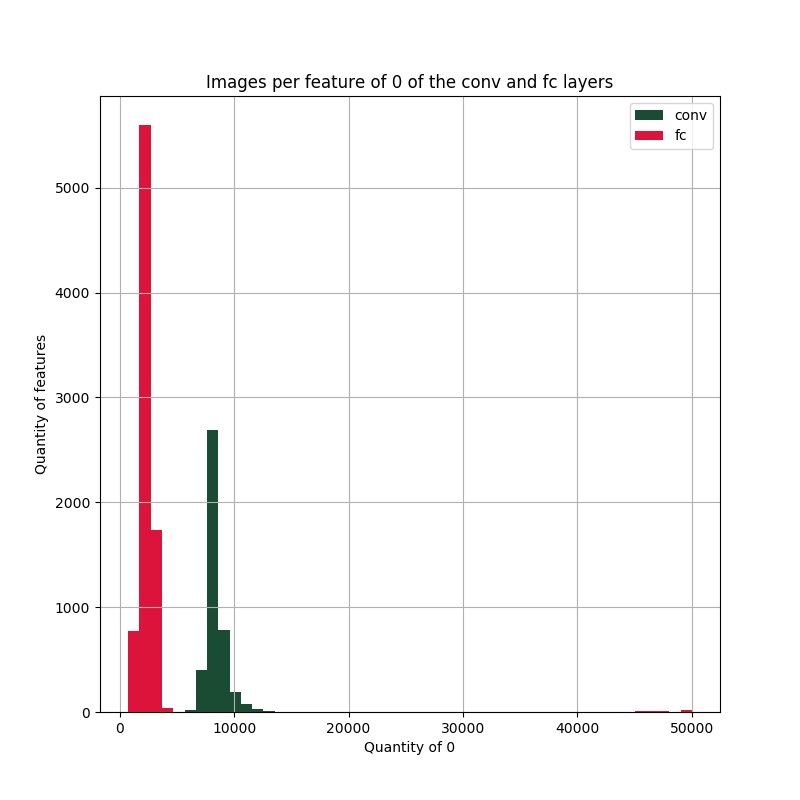
\includegraphics[width=\textwidth]  {Images/plots/25/Images_per_feature_of_0_category_all_layers.png}
		\caption{Categoría 0}
	\end{subfigure}
	\begin{subfigure}[b]{0.32\textwidth}
		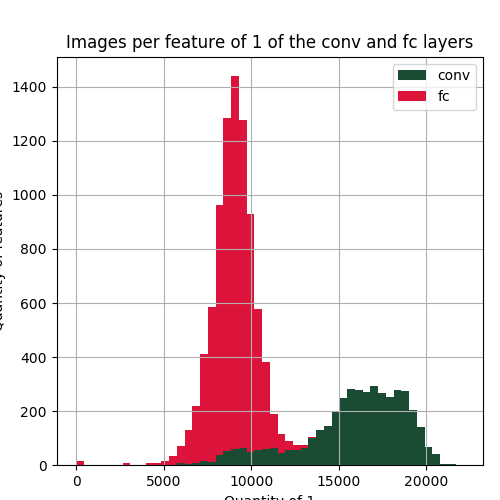
\includegraphics[width=\textwidth]  {Images/plots/25/Images_per_feature_of_1_category_all_layers.png}
		\caption{Categoría 1}
	\end{subfigure}       
	\caption{Distribución del número de \textit{features} con los distintos valores categóricos distinguiendo las capas convolucionales de las \textit{fully-connected}  \label{fig:imagesperfeature}}
\end{figure}


\end{frame}

\begin{frame}{Comportamiento respecto a la profundidad}


\begin{figure}[ht] 
	\centering
	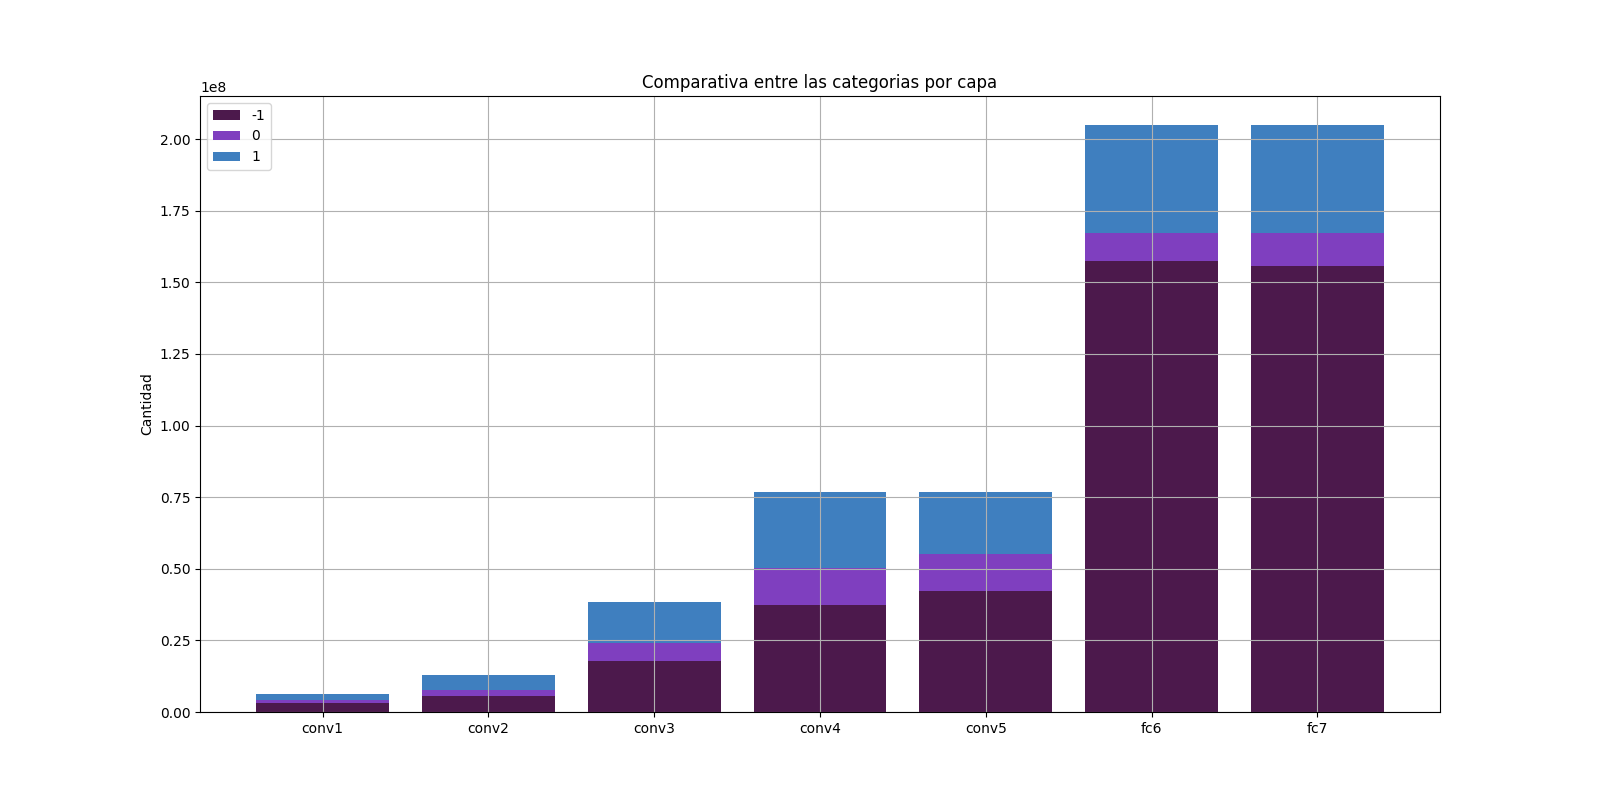
\includegraphics[width=0.9\textwidth] {Images/plots/25/Comparative_of_synsets_all.png}
	
	\resizebox{\linewidth}{!}{% Resize table to fit within \linewidth horizontally

\begin{tabular}{|l|l|l|l|l|l|l|l|l|l|}
\hline
 & conv1 & conv2 & conv3 & conv4 & conv5 & fc6 & fc7 \\ \hline
 Proporción de -1 & 0.47 & 0.44 & 0.46 & 0.49 & 0.55 & 0.77 & 0.76 \\ \hline
 Proporción de 0 & 0.18 & 0.17 & 0.17 & 0.17 & 0.17 & 0.05 & 0.06 \\ \hline
 Proporción de 1 & 0.36 & 0.39 & 0.37 & 0.34 & 0.28 & 0.18 & 0.18 \\ 
\hline
\end{tabular}
}
	\caption{ Cantidad de \textit{features} de cada categoría por capa
	\label{fig:totalfeaturesperlayer}}
\end{figure}



\end{frame}

\subsection{Synset}

\begin{frame}[fragile]{Sub-matriz}
\begin{figure}[H]
\begin{center}
%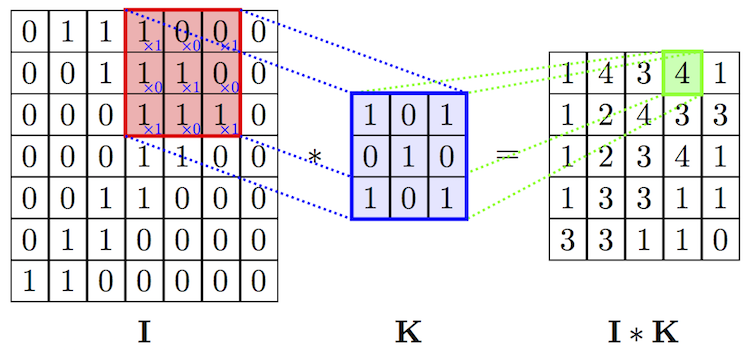
\includegraphics[width = 0.5\textwidth]{Images/convolve.png} 
\begin{tikzpicture}

	\matrix (mtr) [matrix of nodes,column sep=-\pgflinewidth, row sep=-\pgflinewidth,  nodes={draw,
      minimum height=0.5cm,
      anchor=center,
      text width=0.5cm,
      align=center,
      inner sep=0pt
    }]
	{
		|[fill=blue!30]| 1 & |[fill=blue!30]| -1 & |[fill=blue!30]| -1 & |[fill=blue!30]| 1 & |[fill=blue!30]| 0 & |[fill=blue!30]| 0 & |[fill=blue!30]| -1\\
		0 & 0 & -1 & -1 & -1 & 0 & 0\\
		0 & 0 & 0 & 1 & -1 & -1 & 0\\
		|[fill=green!30]| 0 & |[fill=green!30]| 1 & |[fill=green!30]| -1 & |[fill=green!30]| 1 & |[fill=green!30]| 1 & |[fill=green!30]| 0 & |[fill=green!30]| 0\\
		|[fill=blue!30]| 1 & |[fill=blue!30]| 1 & |[fill=blue!30]| -1 & |[fill=blue!30]| 0 & |[fill=blue!30]| -1 & |[fill=blue!30]| 0 & |[fill=blue!30]| 0\\
		0 & 0 & -1 & 1 & 0 & 0 & 0\\
		0 & -1 & 1 & 0 & 0 & 0 & 1\\
		|[fill=blue!30]| 1 & |[fill=blue!30]| 1 & |[fill=blue!30]| 1 & |[fill=blue!30]| -1 & |[fill=blue!30]| -1 & |[fill=blue!30]| 0 & |[fill=blue!30]| 0\\
		-1 & -1 & 0 & 0 & 0 & 0 & 0\\
	};

    \node [below= of mtr-7-4.south] (lm) {embedding};
    

	\matrix (K) [right=5em of mtr,matrix of nodes,row sep=-\pgflinewidth, nodes={draw,minimum height=0.5cm,
      anchor=center,
      text width=0.5cm,
      align=center,
      inner sep=0pt, fill=blue!30}]
	{
		1 & -1 & -1 &  1 &  0 & 0 & -1\\
		1 &  1 & -1 &  0 & -1 & 0 & 0\\
		1 &  1 &  1 & -1 & -1 & 0 & 0\\
	};
    \node [below= of K-2-4.south] (lk) {sub-matriz};

    \draw[very thick, blue] (K-1-1.north west) rectangle (K-3-7.south east);
	
	\draw[densely dotted, blue, thick] (mtr-1-1.north west) -- (K-1-1.north west);
	\draw[densely dotted, blue, thick] (mtr-1-1.south west) -- (K-1-1.south west);
	\draw[densely dotted, blue, thick] (mtr-1-7.north east) -- (K-1-7.north east);
	\draw[densely dotted, blue, thick] (mtr-1-7.south east) -- (K-1-7.south east);
	
	\draw[densely dotted, blue, thick] (mtr-5-1.north west) -- (K-2-1.north west);
	\draw[densely dotted, blue, thick] (mtr-5-1.south west) -- (K-2-1.south west);
	\draw[densely dotted, blue, thick] (mtr-5-7.north east) -- (K-2-7.north east);
	\draw[densely dotted, blue, thick] (mtr-5-7.south east) -- (K-2-7.south east);
	
    \draw[densely dotted, blue, thick] (mtr-8-1.north west) -- (K-3-1.north west);
	\draw[densely dotted, blue, thick] (mtr-8-1.south west) -- (K-3-1.south west);
	\draw[densely dotted, blue, thick] (mtr-8-7.north east) -- (K-3-7.north east);
	\draw[densely dotted, blue, thick] (mtr-8-7.south east) -- (K-3-7.south east);
\end{tikzpicture}
\end{center}
\caption{Ejemplo de una sub-matriz de un \textit{synset}.
\label{fig:submatrix}}
\end{figure}
\end{frame}

\begin{frame}{Distribución por tipo de capa entre los \textit{synsets}}

\begin{figure}[ht] 
	\centering
	\begin{subfigure}[b]{0.32\textwidth}
		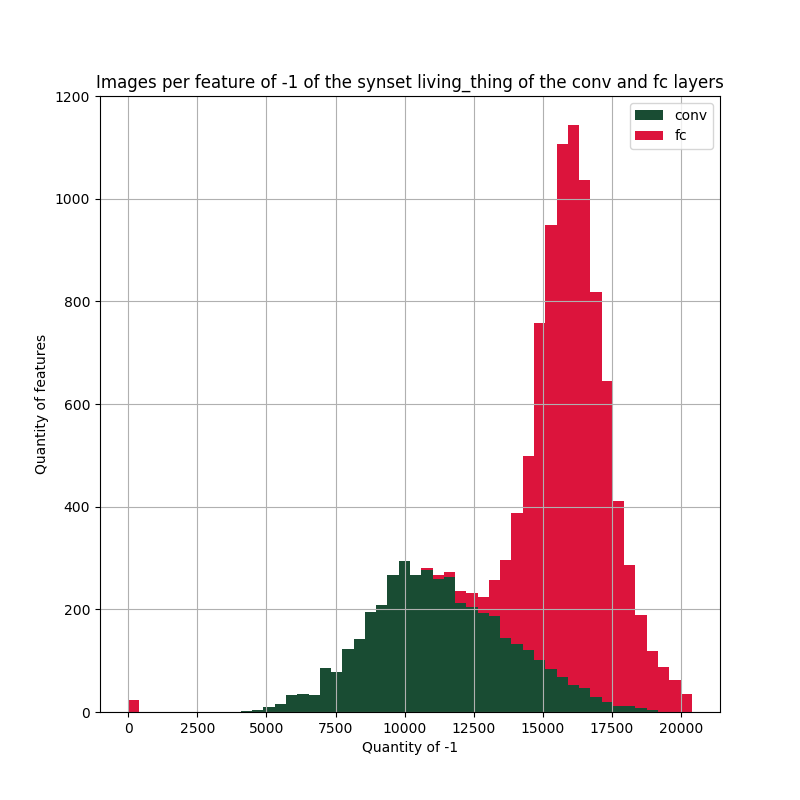
\includegraphics[width=\textwidth] {Images/plots/25/synsets/Images_per_feature_of_-1_category_living_thingall_layers.png}
		\caption{Categoría -1}
	\end{subfigure}
	\begin{subfigure}[b]{0.3\textwidth}
		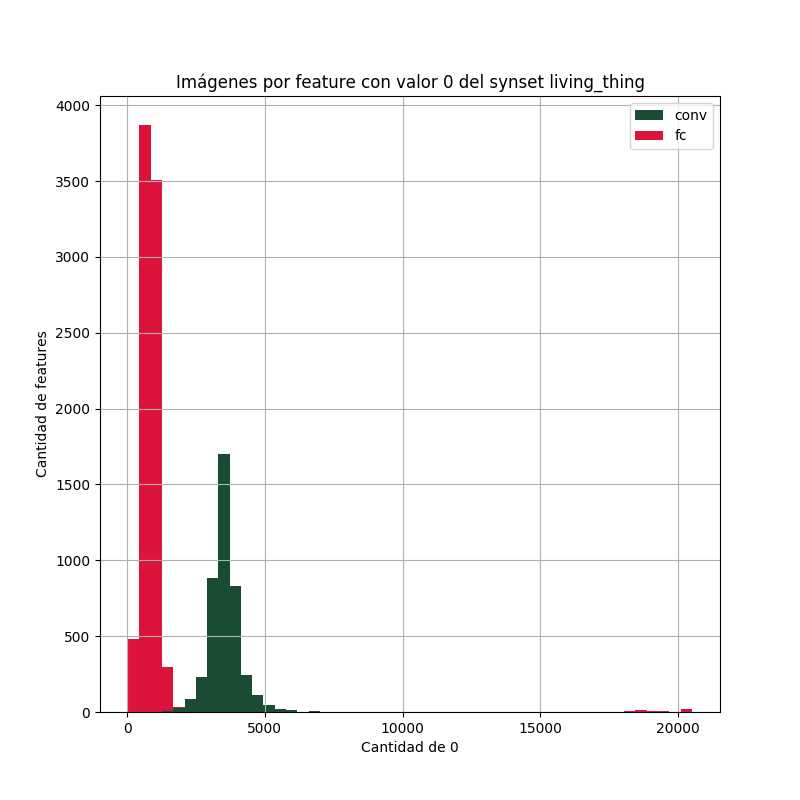
\includegraphics[width=\textwidth]  {Images/plots/25/synsets/Images_per_feature_of_0_category_living_thingall_layers.png}
		\caption{Categoría 0}
	\end{subfigure}
	\begin{subfigure}[b]{0.3\textwidth}
		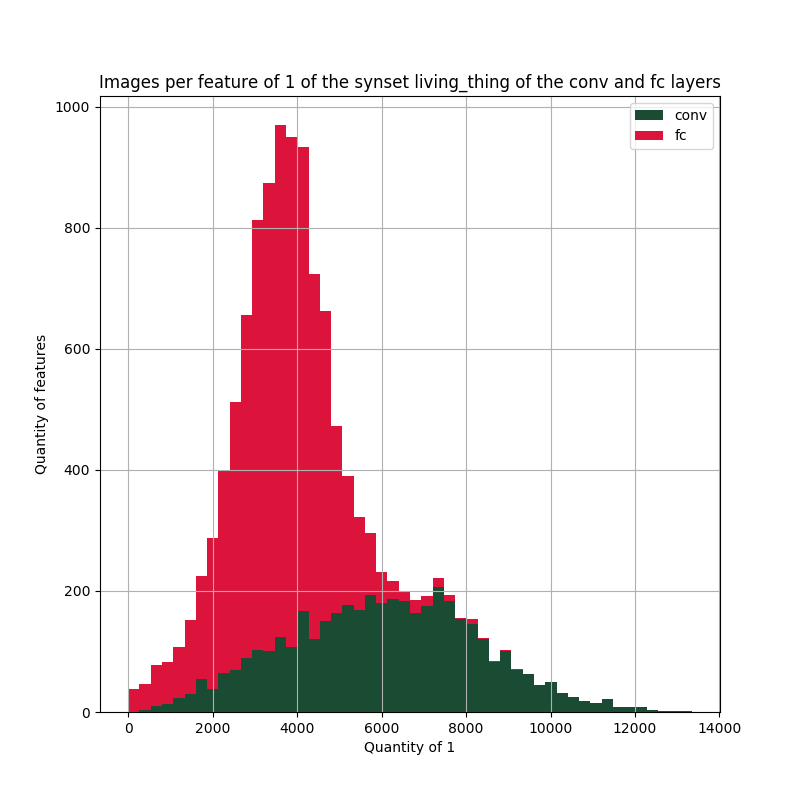
\includegraphics[width=\textwidth]  {Images/plots/25/synsets/Images_per_feature_of_1_category_living_thingall_layers.png}
		\caption{Categoría 1}
	\end{subfigure}       
	\caption{Distribución del número de \textit{features} con los distintos valores categóricos distinguiendo las capas convolucionales de las \textit{fully-connected} del \textit{synset} seres vivos \label{fig:imagesperfeatureliving}}
\end{figure}
\end{frame}

\begin{frame}[fragile]{Distribución de las \textit{features} entre los \textit{synsets}}

\begin{figure}[ht] 
	\centering
	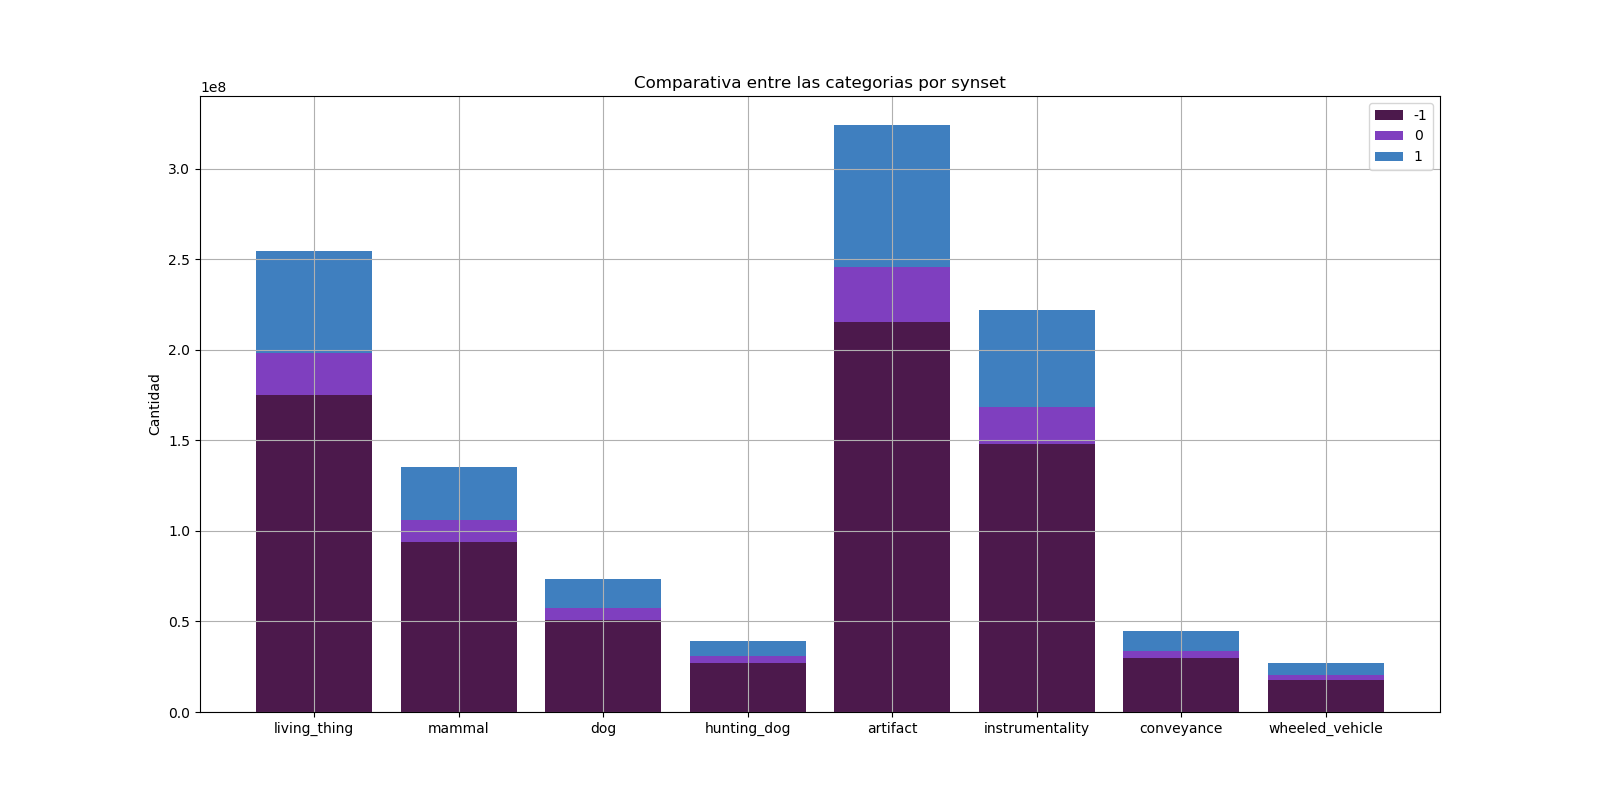
\includegraphics[width=0.9\textwidth] {Images/plots/25/synsetslayer/Comparative_of_synsets_global.png}
	
	\resizebox{\linewidth}{!}{% Resize table to fit within \linewidth horizontally

\begin{tabular}{|l|l|l|l|l|l|l|l|l|l|l|}
\hline
 & Ser Vivo & Mamífero & Perro & Perro de Caza & Artefacto & Instrumento & Transporte & Vehículo \\ \hline
 -1 & 0.69 & 0.69 & 0.70 & 0.70 & 0.66 & 0.67 & 0.66 & 0.65 \\ \hline
  0 & 0.09 & 0.09 & 0.09 & 0.09 & 0.09 & 0.09 & 0.09 & 0.09 \\ \hline
  1 & 0.22 & 0.22 & 0.21 & 0.21 & 0.24 & 0.24 & 0.25 & 0.26 \\
\hline
\end{tabular} }
\caption{ Cantidad y proporción de \textit{features} de cada categoría por synset
	\label{fig:totalfeaturespersynset}}

\end{figure}

\end{frame}

\begin{frame}[fragile]{Representante}

\begin{figure}[ht]
\begin{center}
%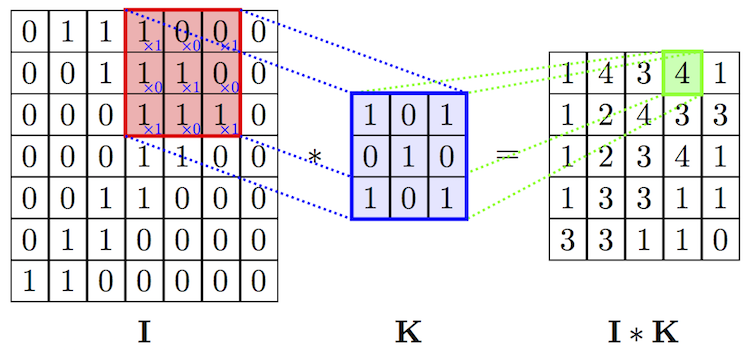
\includegraphics[width = 0.5\textwidth]{Images/convolve.png} 
\begin{tikzpicture}

	\matrix (mtr) [matrix of nodes,column sep=-\pgflinewidth, row sep=-\pgflinewidth,  nodes={draw,
      minimum height=0.5cm,
      anchor=center,
      text width=0.5cm,
      align=center,
      inner sep=0pt
    }]
	{
		|[fill=blue!30]| 1 & |[fill=blue!30]| -1 & |[fill=blue!30]| -1 & |[fill=blue!30]| 1 & |[fill=blue!30]| 0 & |[fill=blue!30]| 0 & |[fill=blue!30]| -1\\
		0 & 0 & -1 & -1 & -1 & 0 & 0\\
		0 & 0 & 0 & 1 & -1 & -1 & 0\\
		|[fill=green!30]| 0 & |[fill=green!30]| 1 & |[fill=green!30]| -1 & |[fill=green!30]| 1 & |[fill=green!30]| 1 & |[fill=green!30]| 0 & |[fill=green!30]| 0\\
		|[fill=blue!30]| 1 & |[fill=blue!30]| 1 & |[fill=blue!30]| -1 & |[fill=blue!30]| 0 & |[fill=blue!30]| -1 & |[fill=blue!30]| 0 & |[fill=blue!30]| 0\\
		0 & 0 & -1 & 1 & 0 & 0 & 0\\
		0 & -1 & 1 & 0 & 0 & 0 & 1\\
		|[fill=blue!30]| 1 & |[fill=blue!30]| 1 & |[fill=blue!30]| 1 & |[fill=blue!30]| -1 & |[fill=blue!30]| -1 & |[fill=blue!30]| 0 & |[fill=blue!30]| 0\\
		-1 & -1 & 0 & 0 & 0 & 0 & 0\\
	};
    \node [below= of mtr-7-4.south] (lm) {embedding};


	\matrix (K) [right=5em of mtr,matrix of nodes,row sep=-\pgflinewidth, nodes={draw, fill=blue!30}]
	{
		1 & 1 & -1 & 1 & -1 & 0 & 0\\
	};
	
    \node [below= of K-1-4.south] (lk) {representante};

    \draw[very thick, blue] (K-1-1.north west) rectangle (K-1-7.south east);
	
	\draw[densely dotted, blue, thick] (mtr-1-1.north west) -- (K-1-1.north west);
	\draw[densely dotted, blue, thick] (mtr-1-1.south west) -- (K-1-1.south west);
	\draw[densely dotted, blue, thick] (mtr-1-7.north east) -- (K-1-7.north east);
	\draw[densely dotted, blue, thick] (mtr-1-7.south east) -- (K-1-7.south east);
	
	\draw[densely dotted, blue, thick] (mtr-5-1.north west) -- (K-1-1.north west);
	\draw[densely dotted, blue, thick] (mtr-5-1.south west) -- (K-1-1.south west);
	\draw[densely dotted, blue, thick] (mtr-5-7.north east) -- (K-1-7.north east);
	\draw[densely dotted, blue, thick] (mtr-5-7.south east) -- (K-1-7.south east);
	
    \draw[densely dotted, blue, thick] (mtr-8-1.north west) -- (K-1-1.north west);
	\draw[densely dotted, blue, thick] (mtr-8-1.south west) -- (K-1-1.south west);
	\draw[densely dotted, blue, thick] (mtr-8-7.north east) -- (K-1-7.north east);
	\draw[densely dotted, blue, thick] (mtr-8-7.south east) -- (K-1-7.south east);
%	\draw[very thick, blue] (K-1-1.north west) rectangle (K-3-3.south east);

\end{tikzpicture}
\end{center}
\caption{Ejemplo de un representante de \textit{synset}.
\label{fig:representante}}
\end{figure}

\end{frame}

\begin{frame}{Distribución de las \textit{features} entre los representantes}
\begin{figure}[ht] 
	\centering
	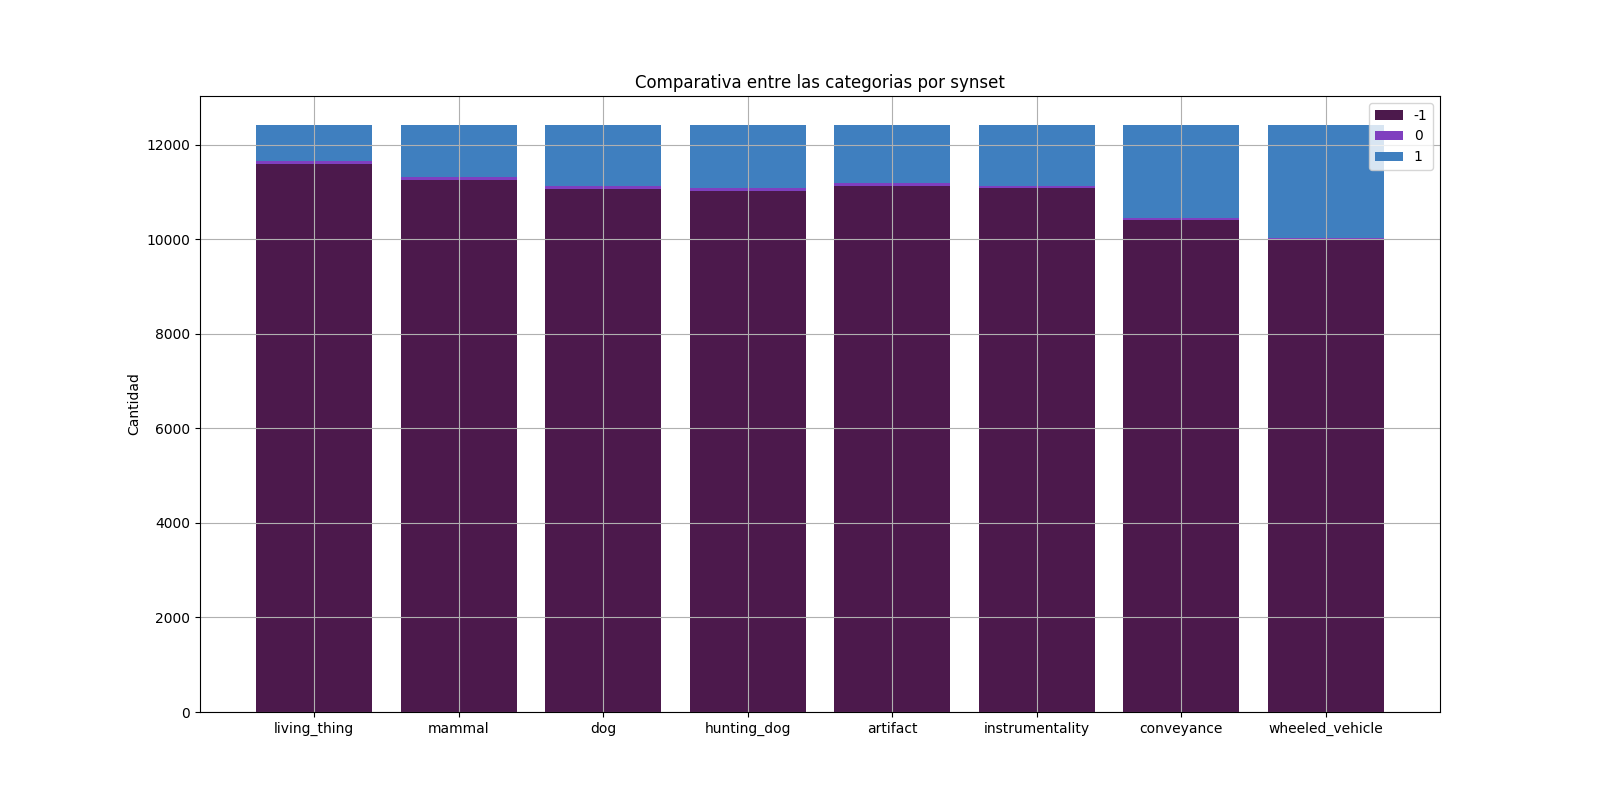
\includegraphics[width=0.9\textwidth] {Images/plots/25/synsetslayer/Comparative_of_synsets.png}
	\caption{ Cantidad de \textit{features} de cada tipo de los representantes de los distintos \textit{synsets}
	\label{fig:comparativaCategoriasporSynset}}
\end{figure}
\end{frame}

\begin{frame}{Distribución de las \textit{features} entre los representantes por capa}
\begin{figure}[ht] 
	\centering
	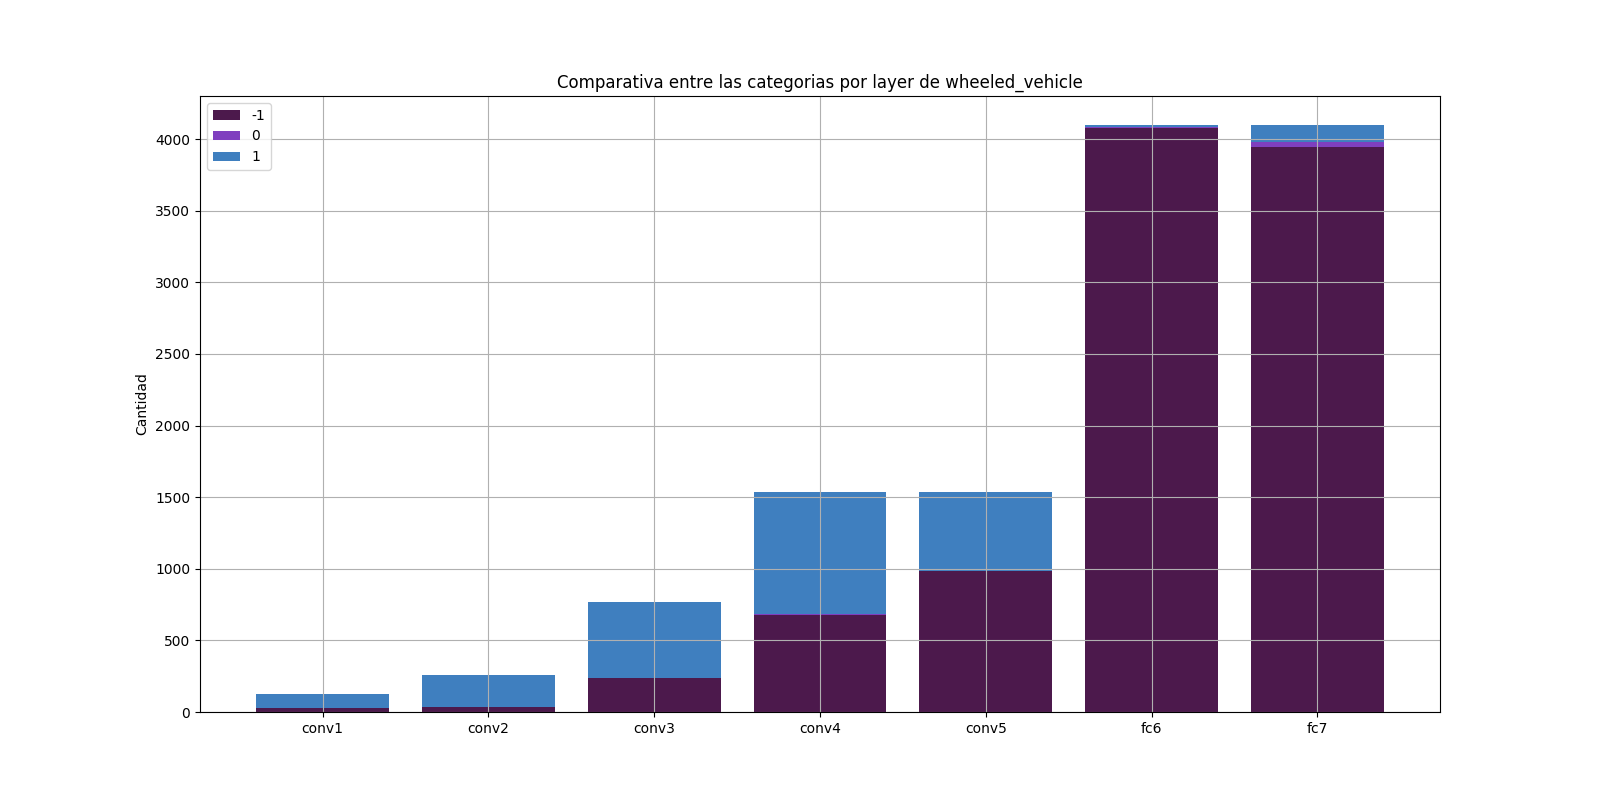
\includegraphics[width=0.9\textwidth] {Images/plots/25/synsetslayer/Comparative_of_synsets_wheeled_vehicle.png}
	\caption{ Cantidad de \textit{features} de cada tipo del representante del \textit{synset} Vehículo por capa.
	\label{fig:comparativaVehiculo}}
\end{figure}
\end{frame}




\subsection{De Full-Network Embedding a Wordnet}
\begin{frame}{Matrices de cambio}
 \begin{figure}[ht] 
	\centering
	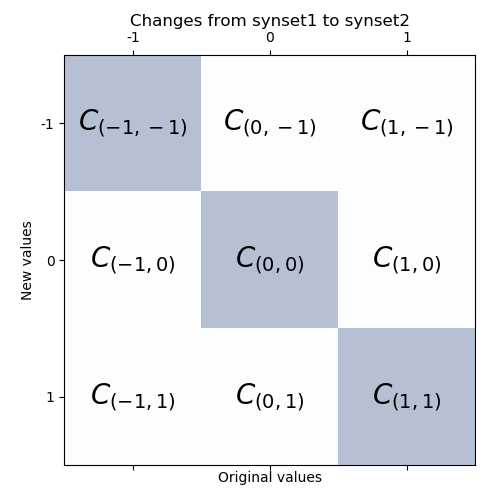
\includegraphics[width=0.55\textwidth] {Images/plots/25/matrices/Changesfromsynset1tosynset2.png}
	\caption{ Matriz de cambios general
	\label{fig:matrizss1ss2}}
\end{figure}
\end{frame}

%\begin{frame}{Ejemplo}
% \begin{figure}[ht] 
%	\centering
%	\begin{subfigure}[b]{0.3\textwidth}
%		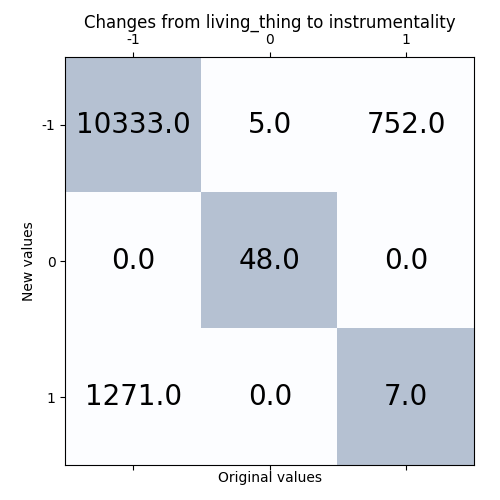
\includegraphics[width=\textwidth] {Images/plots/25/matrices/matrixlivinginstrum.png}
%		\caption{Ser Vivo a Instrumento \label{fig:matrixlivinginstrum}}
%	\end{subfigure}
%	\begin{subfigure}[b]{0.3\textwidth}
%		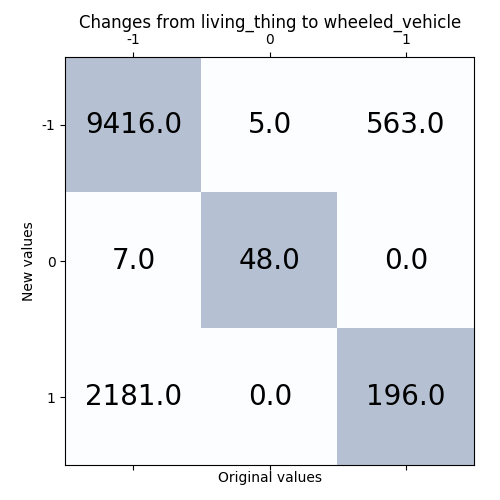
\includegraphics[width=\textwidth]  {Images/plots/25/matrices/matrixLivingWheel.png}
%		\caption{Ser Vivo a Vehículo \label{fig:matrixlivingwheel}}
%	\end{subfigure}
%	\begin{subfigure}[b]{0.3\textwidth}
%		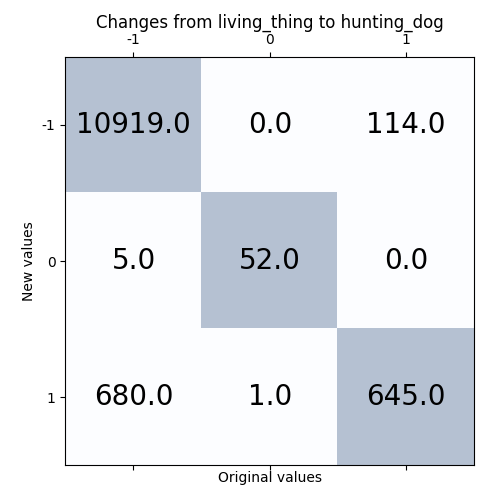
\includegraphics[width=\textwidth]  {Images/plots/25/matrices/matrixLivingHunting.png}
%		\caption{Ser Vivo a Perro de Caza \label{fig:matrixlivinghunting}}
%	\end{subfigure}       
%	\caption{Matrices de cambio de Ser Vivo \label{fig:matrixliving}}
%\end{figure}
%\end{frame}


\begin{frame}{Pseudo-Métrica}
% Todo: poner esto mono
\begin{equation*}
\resizebox{\linewidth}{!}{$\displaystyle % restart math mode
T = C_{(1,-1)}(s_1,s_2) + C_{(1,0)}(s_1,s_2) + C_{(1,1)}(s_1,s_2) + C_{(1,1)}(s_1,s_2) + C_{(0,1)}(s_1,s_2) + C_{(-1,1)}(s_1,s_2) 
$}
\end{equation*}
\begin{align*}
d(s_1,s_2) = 1 - \frac{C_{(1,1)}(s_1,s_2)}{T}
\end{align*}
\begin{table}[]
\centering

\begin{tabular}{l|l|l|l}
           & Instrumento & Vehículo & Perro de Caza               \\ \hline
Ser Vivo   & 0.9965      & 0.9333   & \multicolumn{1}{l|}{0.5520} \\ \hline
Perro      & 0.9671      & 0.8753   & \multicolumn{1}{l|}{0.1614} \\ \hline
Transporte & 0.2201      & 0.2192   & \multicolumn{1}{l|}{0.9124} \\ \cline{2-4} 
\end{tabular}
\end{table}
\end{frame}

%\begin{frame}

%\begin{figure}[ht] 
%	\centering
%	\begin{subfigure}[b]{0.3\textwidth}
%		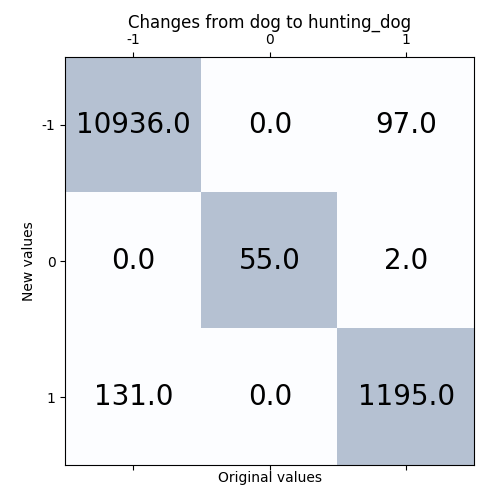
\includegraphics[width=\textwidth] {Images/plots/25/matrices/MatrixDogHunting.png}
%		\caption{Perro a Perro de caza \label{fig:MatrixDogHunting}}
%	\end{subfigure}
%	\begin{subfigure}[b]{0.3\textwidth}
%		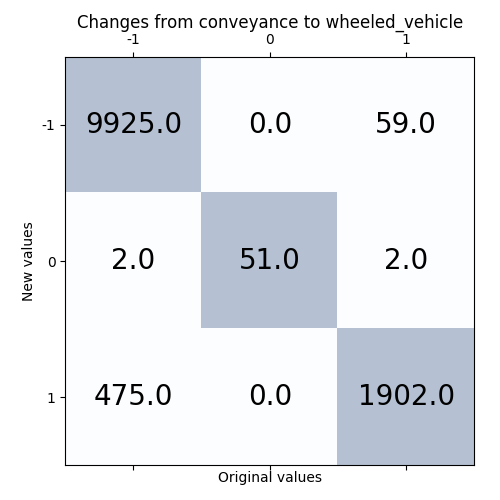
\includegraphics[width=\textwidth]  {Images/plots/25/matrices/matrixConveyanceWheel.png}
%		\caption{Transporte a Vehículo \label{fig:matrixConveyanceWheel}}
%	\end{subfigure}
%	\begin{subfigure}[b]{0.3\textwidth}
%		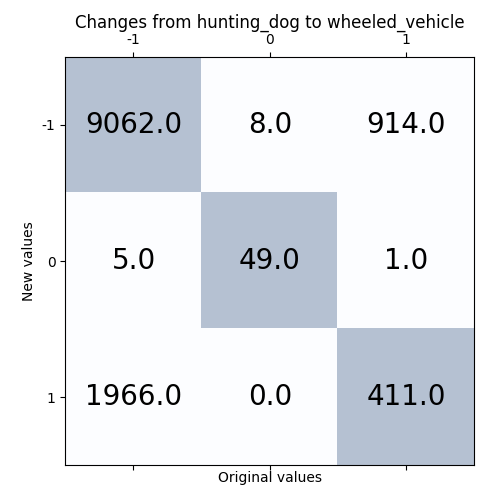
\includegraphics[width=\textwidth]  {Images/plots/25/matrices/matrixhuntingwheel.png}
%		\caption{Perro de caza a Vehículo\label{fig:MatrixWheelHunt}}
%	\end{subfigure}       
%	\caption{Matrices de cambio\label{fig:matrixconcret}}
%\end{figure}
%\end{frame}


\begin{frame}{Ejemplos}

\begin{figure}[H] 
	\centering
	\begin{subfigure}[b]{0.3\textwidth}
		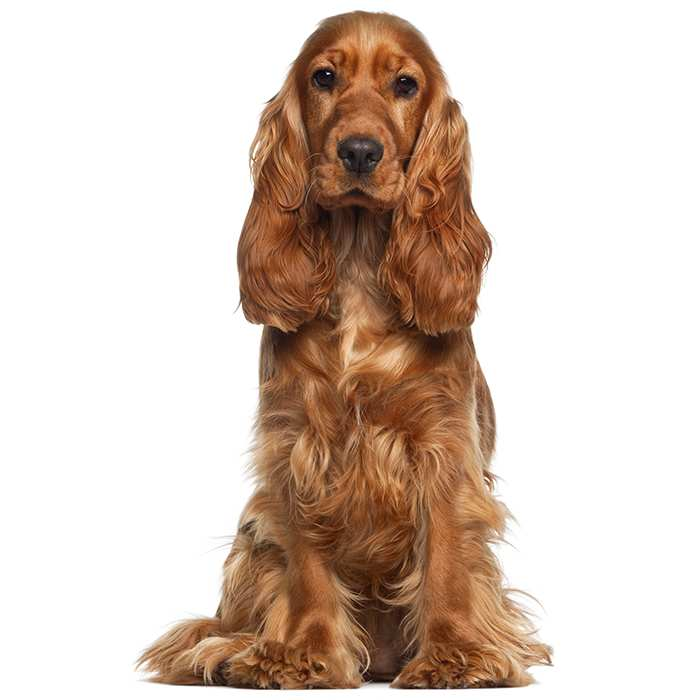
\includegraphics[height=3cm] {Images/examples/spaniel.jpg}
		\caption{Spaniel \label{fig:spaniel}}
	\end{subfigure}
	\begin{subfigure}[b]{0.3\textwidth}
		\centering
		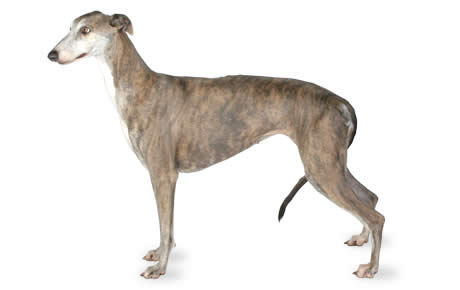
\includegraphics[height=3cm]  {Images/examples/greyhound.jpg}
		\caption{Greyhound \label{fig:greyhound}}
	\end{subfigure}
	\begin{subfigure}[b]{0.3\textwidth}
		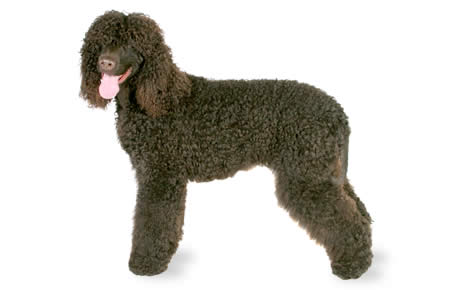
\includegraphics[height=3cm]{Images/examples/waterspaniel.jpg}
		\caption{Water Spaniel\label{fig:waterspaniel}}
	\end{subfigure}       
	\caption{Ejemplos de razas\label{fig:dogexample}}
\end{figure}

\begin{table}[H]
\centering
%\caption{Distancias entre las razas del ejemplo}
%\label{tabledogs}
\begin{tabular}{l|l|l|l}
              & Spaniel & Grayhound & Water Spaniel               \\ \hline
Spaniel       & 0       & 0.7371    & \multicolumn{1}{l|}{0.6442} \\ \hline
Grayhound     & 0.7371  & 0         & \multicolumn{1}{l|}{0.8330} \\ \hline
Water Spaniel & 0.6442  & 0.8330    & \multicolumn{1}{l|}{0}      \\ \cline{2-4} 
\end{tabular}
\end{table}
\end{frame}

\begin{frame}
 \begin{figure}[H] 
	\centering
	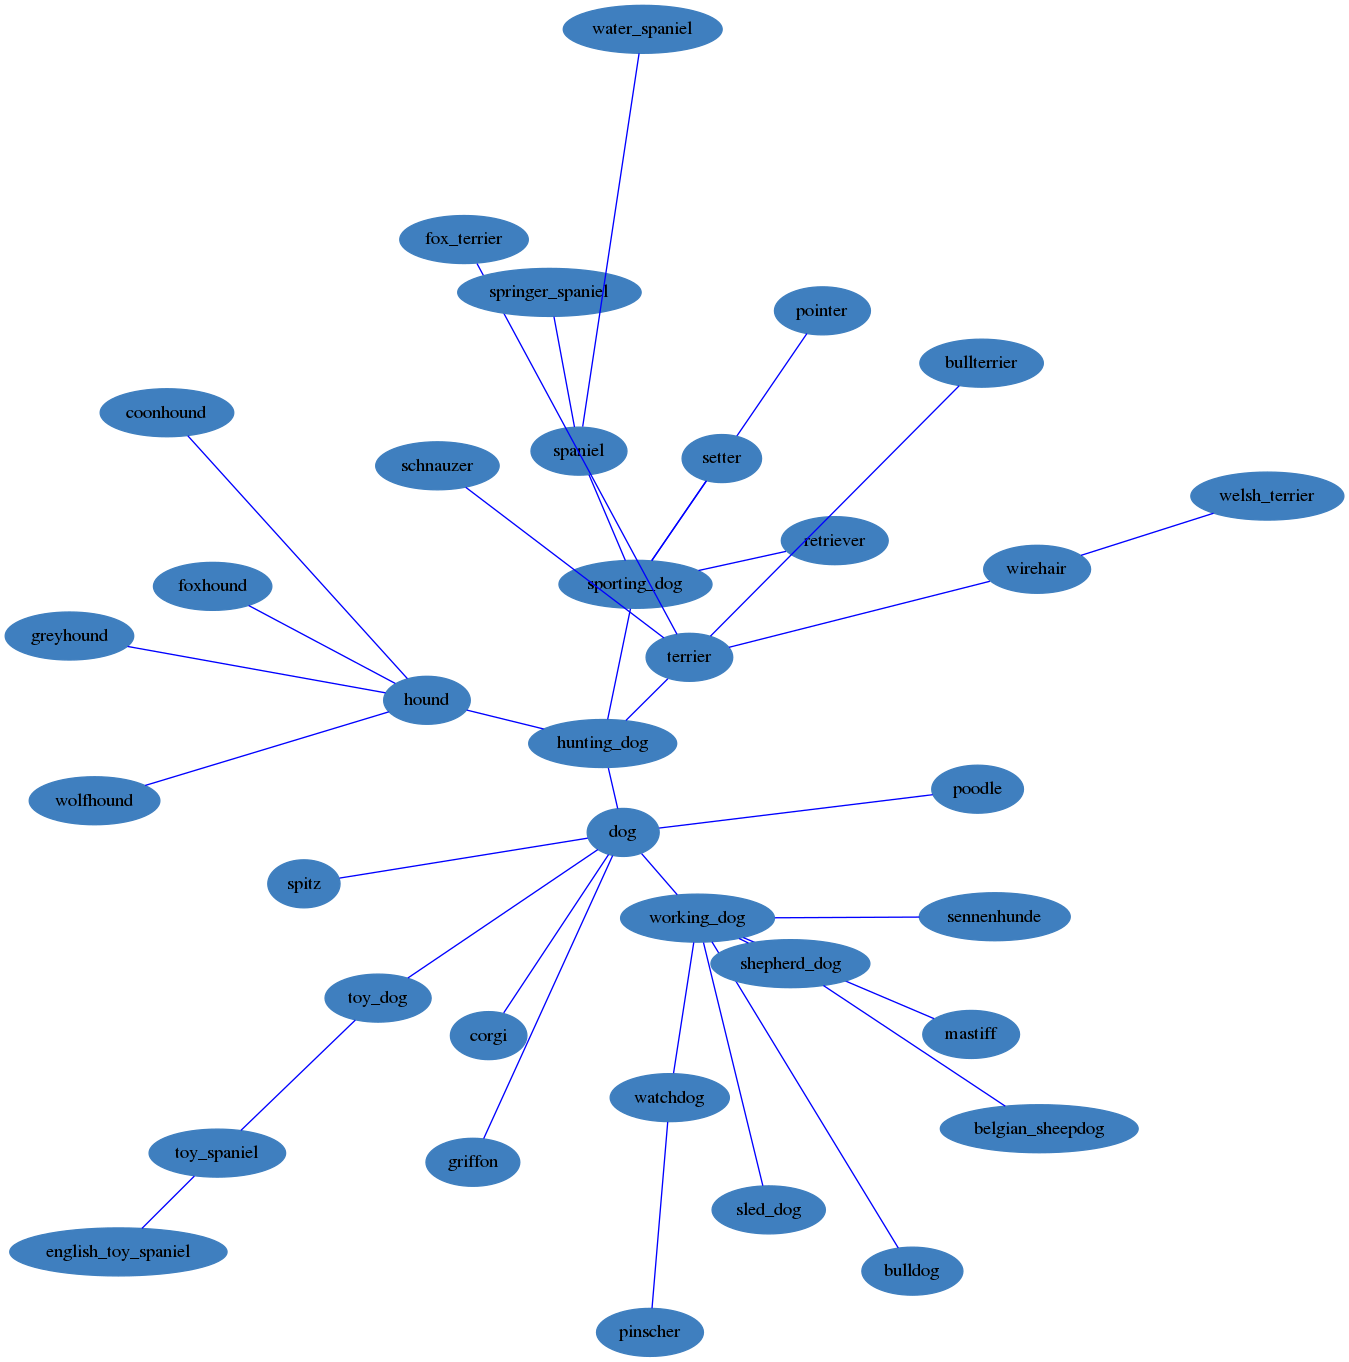
\includegraphics[height=0.8\textheight] {Images/forest/dog.png}
	\caption{Ejemplo de Árbol del \textit{synset} perro con distancias normalizadas según la métrica comentada. 
	\label{fig:grafoperro}}
\end{figure}

\end{frame}
% Placing a * after \section means it will not show in the
% outline or table of contents.

\section{Conclusiones}
\begin{frame}{Conclusiones}
\begin{itemize}
\item Las capas \textit{fully-connected} tienen una distribución diferente de las convolucionales.
\item Todas las \textit{features} contienen información que caracteriza el espacio de representación. 
\item Las proporciones de las \textit{features} se mantienen respecto a las profundidad de las capas.
\item La proporción de las \textit{features} de las tres categorías se mantiene respecto a los diferentes synsets. 
\item El \textit{embedding} detecta similitud a nivel de \textit{synset}. 
\item Utilizando la pseudo-métrica definida podemos medir esta distancia y representarla gráficamente. 
\end{itemize}
\end{frame}
\section*{}
\begin{frame}
    \centering
    \begin{huge}
    Gracias por vuestra atención.
    \end{huge}
        
        
        %\url{https://github.com/RaquelLeandra/TFG-WordnetDeepLearning}
    \begin{figure}
     \includegraphics[width=0.7\textwidth]{Images/github-octocat.png}
    \end{figure}
    Podéis encontrar el código utilizado en el trabajo en:
    \url{github.com/RaquelLeandra/TFG-WordnetDeepLearning}
   \end{frame}



\end{document}


